\documentclass[aspectratio=169]{beamer}

% ── Theme & Colors ──────────────────────────────────────────
\usetheme{Madrid}
\usecolortheme{default}

\definecolor{darkblue}{RGB}{26, 54, 93}
\definecolor{accentblue}{RGB}{52, 101, 164}
\definecolor{lightgray}{RGB}{245, 245, 245}
\definecolor{alertred}{RGB}{192, 57, 43}
\definecolor{okgreen}{RGB}{39, 174, 96}
\definecolor{warnorange}{RGB}{230, 126, 34}

\setbeamercolor{palette primary}{bg=darkblue, fg=white}
\setbeamercolor{palette secondary}{bg=accentblue, fg=white}
\setbeamercolor{palette tertiary}{bg=darkblue, fg=white}
\setbeamercolor{palette quaternary}{bg=darkblue, fg=white}
\setbeamercolor{structure}{fg=darkblue}
\setbeamercolor{section in toc}{fg=darkblue}
\setbeamercolor{frametitle}{bg=darkblue, fg=white}
\setbeamercolor{title}{bg=darkblue, fg=white}
\setbeamercolor{block title}{bg=accentblue, fg=white}
\setbeamercolor{block body}{bg=lightgray, fg=black}
\setbeamercolor{alertblock title}{bg=alertred, fg=white}
\setbeamercolor{alerted text}{fg=alertred}

% ── Packages ────────────────────────────────────────────────
\usepackage{graphicx}
\usepackage{booktabs}
\usepackage{tikz}
\usetikzlibrary{positioning}
\usepackage{amsmath}
\usepackage{xcolor}
\usepackage{array}
\usepackage{colortbl}

% ── Custom commands ─────────────────────────────────────────
\newcommand{\highlight}[1]{\textcolor{accentblue}{\textbf{#1}}}
\newcommand{\good}[1]{\textcolor{okgreen}{\textbf{#1}}}
\newcommand{\bad}[1]{\textcolor{alertred}{\textbf{#1}}}
\newcommand{\warn}[1]{\textcolor{warnorange}{\textbf{#1}}}

% ── Footer ──────────────────────────────────────────────────
\setbeamertemplate{footline}{
	\leavevmode
	\hbox{%
		\begin{beamercolorbox}[wd=.33\paperwidth,ht=2.25ex,dp=1ex,center]{palette primary}%
			\usebeamerfont{author in head/foot}AI354: Responsible AI
		\end{beamercolorbox}%
		\begin{beamercolorbox}[wd=.34\paperwidth,ht=2.25ex,dp=1ex,center]{palette secondary}%
			\usebeamerfont{title in head/foot}Project 10
		\end{beamercolorbox}%
		\begin{beamercolorbox}[wd=.33\paperwidth,ht=2.25ex,dp=1ex,right]{palette tertiary}%
			\usebeamerfont{date in head/foot}
			\insertframenumber{} / \inserttotalframenumber\hspace*{2ex}
	\end{beamercolorbox}}%
	\vskip0pt%
}
\setbeamertemplate{navigation symbols}{}

% ── Title Info ───────────────────────────────────────────────
\title[Data Poisoning Attacks]{\textbf{Detecting and Preventing\\Data Poisoning Attacks}}
\subtitle{Project 10: AI354 Responsible AI}
\author[Chauhan \& Gawas]{
	\textbf{I23MA002} \ Devesh Singh Chauhan \quad
	\textbf{U23EE102} \ Priyanshu Sanjay Gawas
}
\institute[]{Department of AI, SVNIT}
\date{\today}

% ────────────────────────────────────────────────────────────
\begin{document}
	
	% ── SLIDE 1: Title ──────────────────────────────────────────
	\begin{frame}
		\titlepage

	\end{frame}
	
	% ── SLIDE 2: Problem Statement ──────────────────────────────
	\begin{frame}{Problem Statement}
		\begin{block}{What is Data Poisoning?}
			Data poisoning is an adversarial attack where an attacker \highlight{injects malicious
				or manipulated samples into a model's training data}, causing the model to behave
			incorrectly at inference time.
		\end{block}
		
		\vspace{0.4em}
		\begin{columns}[T]
			\column{0.48\textwidth}
			\textbf{The Core Threat}
			\begin{itemize}\setlength{\itemsep}{0pt}
				\item Attacker controls part of training data
				\item Labels are \bad{flipped} or features \bad{perturbed}
				\item Backdoor triggers inserted silently
				\item Model \bad{appears normal} until triggered
			\end{itemize}
			
			\column{0.48\textwidth}
			\textbf{What We Need}
			\begin{itemize}\setlength{\itemsep}{0pt}
				\item Statistical \highlight{detection} of suspicious samples
				\item \highlight{Robust} training algorithms
				\item Automated \highlight{alerting} pipelines
				\item Validation on \highlight{image} and \highlight{text} models
			\end{itemize}
		\end{columns}
		
		\vspace{0.6em}
		\begin{alertblock}{Key Challenge}
			Poisoned data often \textbf{looks perfectly normal} to a human reviewer; therefore,
			detection must be algorithmic and automated.
		\end{alertblock}
	\end{frame}
	
	% ── SLIDE 3: Motivation ─────────────────────────────────────
	\begin{frame}{Motivation}
		\begin{columns}[T]
			\column{0.55\textwidth}
			\textbf{Why does this matter?}
			\begin{itemize}
				\item ML models are deployed in \highlight{safety-critical systems}:
				autonomous vehicles, medical diagnosis, fraud detection
				\item Training data is often sourced from \bad{untrusted} third parties
				\item A 10\% label-flip attack can drop accuracy by \bad{6-9\%}, which is
				enough to cause real harm
				\item \highlight{Supply-chain attacks} on AI are rising
			\end{itemize}
			
			\vspace{0.5em}
			\begin{block}{Real-World Incidents}
				\begin{itemize}
					\item Microsoft Tay chatbot (2016): poisoned via user input
					\item Trojan attacks on ImageNet classifiers (2018)
					\item NLP backdoor attacks on sentiment analysis (2020+)
				\end{itemize}
			\end{block}
			
			\column{0.42\textwidth}
			\centering
			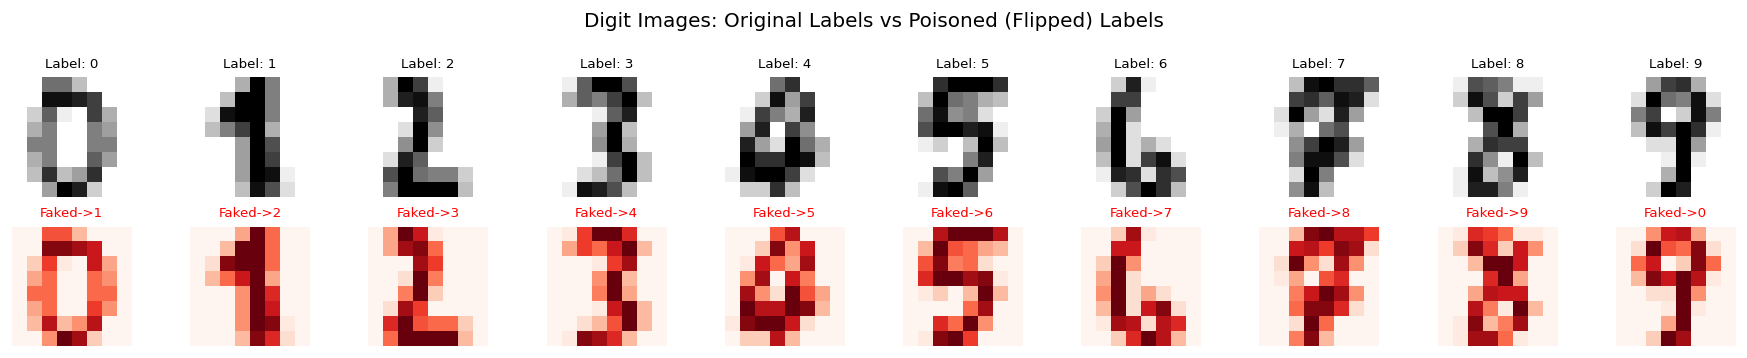
\includegraphics[width=\linewidth,height=0.6\textheight,keepaspectratio]{images/poisoned_images.png}
			\vspace{0.2em}
			
			{\small\textit{Same image, different label: the attacker's trick}}
		\end{columns}
	\end{frame}
	
	% ── SLIDE 4: Attack Types ────────────────────────────────────
	\begin{frame}{Types of Data Poisoning Attacks}
		\begin{columns}[T]
			\column{0.48\textwidth}
			\textbf{\highlight{Label Flipping (Implemented)}}
			\begin{itemize}\setlength{\itemsep}{0pt}
				\item Attacker changes the \textbf{ground-truth labels} of training samples.
				\item E.g., Digit ``8'' labelled as ``4''.
				\item Simple but highly effective at scale.
			\end{itemize}
			
			\vspace{0.8em}
			\textbf{\highlight{Backdoor / Trojan Attack}}
			\begin{itemize}\setlength{\itemsep}{0pt}
				\item A hidden \textbf{trigger pattern} causes misclassification only when present at inference.
			\end{itemize}
			
			\column{0.48\textwidth}
			\textbf{\highlight{Clean-Label Poisoning}}
			\begin{itemize}\setlength{\itemsep}{0pt}
				\item Labels are kept \textbf{correct} but feature vectors are perturbed. Much harder to detect.
			\end{itemize}
			
			\vspace{0.8em}
			\textbf{\highlight{Feature Collision}}
			\begin{itemize}\setlength{\itemsep}{0pt}
				\item Poisoned samples are crafted to be \textbf{close in feature space} to a target class.
			\end{itemize}
		\end{columns}
		
		\vspace{1.2em}
		\begin{alertblock}{Our Focus}
			\textbf{Label-flipping attack}: most common, clearly measurable, and a strong foundation for defense design.
		\end{alertblock}
	\end{frame}
	
	% ── SLIDE 5: Approach & Architecture ────────────────────────
	\begin{frame}{Approach \& System Architecture}
		\begin{center}
			\resizebox{0.95\linewidth}{!}{
				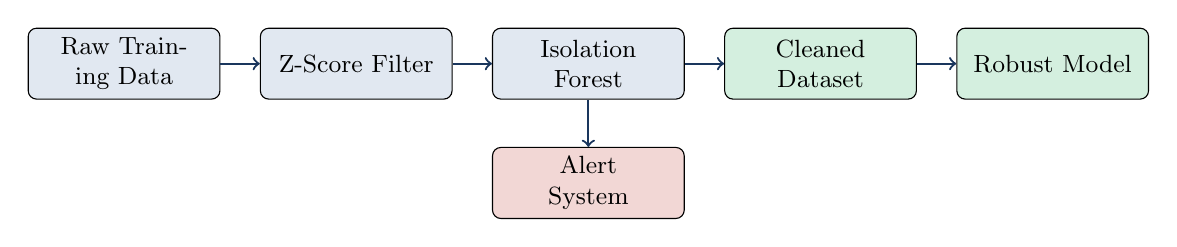
\begin{tikzpicture}[
					node distance=0.6cm and 0.5cm,
					box/.style={draw, rounded corners=3pt, fill=accentblue!15, text width=2.2cm,
						align=center, font=\small, minimum height=0.9cm},
					alert/.style={draw, rounded corners=3pt, fill=alertred!20, text width=2.2cm,
						align=center, font=\small, minimum height=0.9cm},
					good/.style={draw, rounded corners=3pt, fill=okgreen!20, text width=2.2cm,
						align=center, font=\small, minimum height=0.9cm},
					arr/.style={->, thick, darkblue}
					]
					\node[box]  (raw)    {Raw Training Data};
					\node[box]  (zscore) [right=of raw]   {Z-Score Filter};
					\node[box]  (iso)    [right=of zscore]{Isolation Forest};
					\node[alert](alert)  [below=of iso]   {Alert \\ System};
					\node[good] (clean)  [right=of iso]   {Cleaned Dataset};
					\node[good] (model)  [right=of clean] {Robust Model};
					
					\draw[arr] (raw)    -- (zscore);
					\draw[arr] (zscore) -- (iso);
					\draw[arr] (iso)    -- (alert);
					\draw[arr] (iso)    -- (clean);
					\draw[arr] (clean)  -- (model);
				\end{tikzpicture}
			}
		\end{center}
		
		\vspace{0.4em}
		\begin{columns}[T]
			\column{0.32\textwidth}
			\begin{block}{Step 1: Z-Score}
				\small Flag samples where any feature deviates $>2.5\sigma$. Fast, interpretable first pass.
			\end{block}
			\column{0.32\textwidth}
			\begin{block}{Step 2: Isolation Forest}
				\small Unsupervised detection. Isolates subtle cluster-level anomalies via random splits.
			\end{block}
			\column{0.32\textwidth}
			\begin{block}{Step 3: Alerting}
				\small Combined flags trigger a severity-graded alert (\good{OK}/\warn{WARN}/\bad{CRIT}).
			\end{block}
		\end{columns}
	\end{frame}
	
	% ── SLIDE 6: Implementation Details ─────────────────────────
	\begin{frame}{Implementation Details}
		\footnotesize 
		\begin{columns}[T]
			\column{0.48\textwidth}
			\textbf{Image Model}
			\begin{itemize}\setlength{\itemsep}{0pt}
				\item \textbf{Dataset:} sklearn Digits (1797 samples)
				\item \textbf{Attack:} 10\% random label-flip
				\item \textbf{Model:} Logistic Regression
				\item \textbf{Defense:} Isolation Forest (\texttt{cont=0.10})
				\item Features standardized
			\end{itemize}
			
			\vspace{0.4em}
			\textbf{Text Model}
			\begin{itemize}\setlength{\itemsep}{0pt}
				\item \textbf{Dataset:} Synthetic corpus (600 docs)
				\item \textbf{Features:} TF-IDF (500 features)
				\item \textbf{Attack:} 20\% label-flip
				\item \textbf{Defense:} Isolation Forest (\texttt{cont=0.20})
			\end{itemize}
			
			\column{0.48\textwidth}
			\textbf{Tech Stack}
			\begin{itemize}\setlength{\itemsep}{0pt}
				\item Python 3.11, Jupyter Notebook
				\item \texttt{scikit-learn}: models \& detection
				\item \texttt{scipy.stats.zscore}: statistical filter
			\end{itemize}
			
			\vspace{0.4em}
			\begin{block}{DataPoisoningDetector Class}
				Custom Python wrapper with:
				\begin{itemize}\setlength{\itemsep}{0pt}
					\item \texttt{fit(X)}: calibrate on training data
					\item \texttt{scan(X)}: flag suspicious samples
					\item \texttt{clean(X, y)}: return filtered dataset
				\end{itemize}
			\end{block}
		\end{columns}
	\end{frame}
	
	% ── SLIDE 7: Detection Results ───────────────────────────────
	\begin{frame}{Detection Results}
		\begin{columns}[T]
			\column{0.48\textwidth}
			\centering
			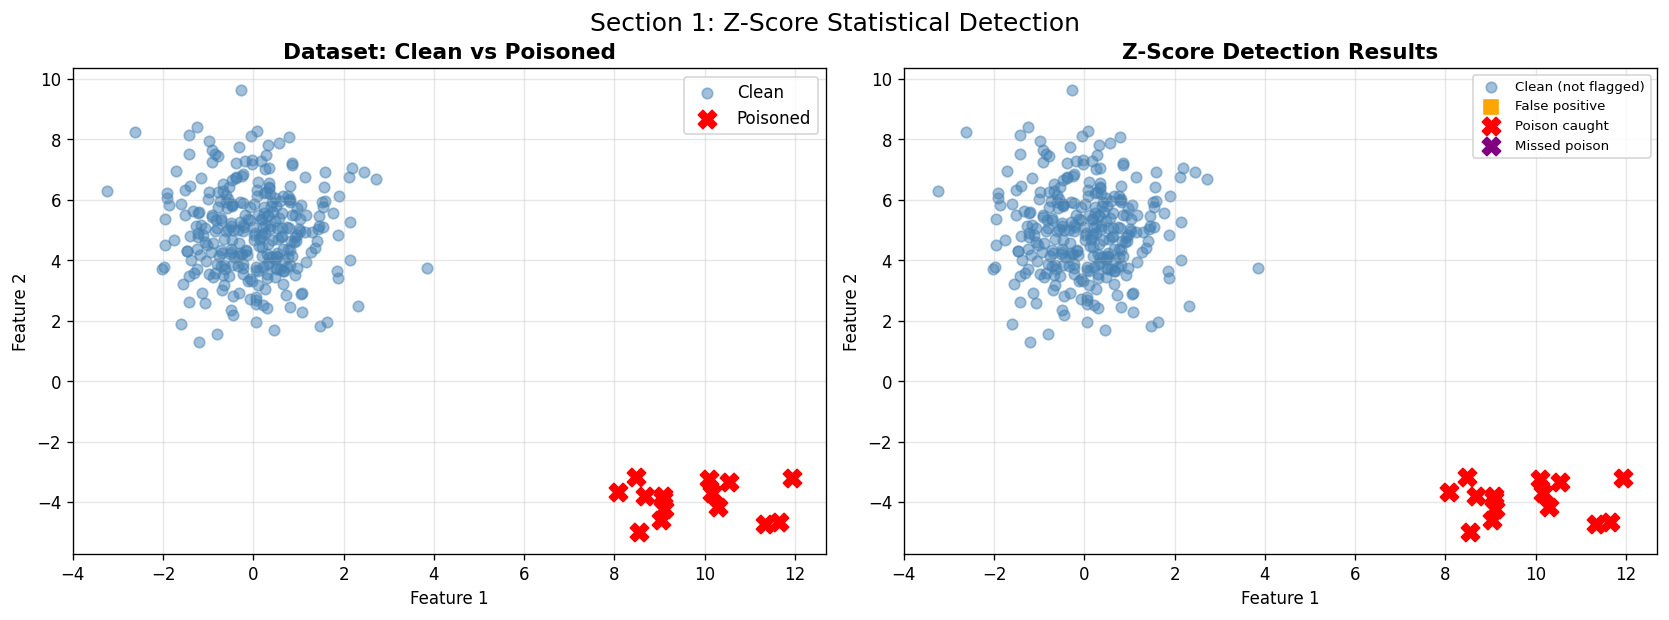
\includegraphics[width=\linewidth,height=0.35\textheight,keepaspectratio]{images/zscore_detection.png}
			
			{\small \textbf{Z-Score:} 100\% detection on synthetic outliers (15/15)}
			
			\column{0.48\textwidth}
			\centering
			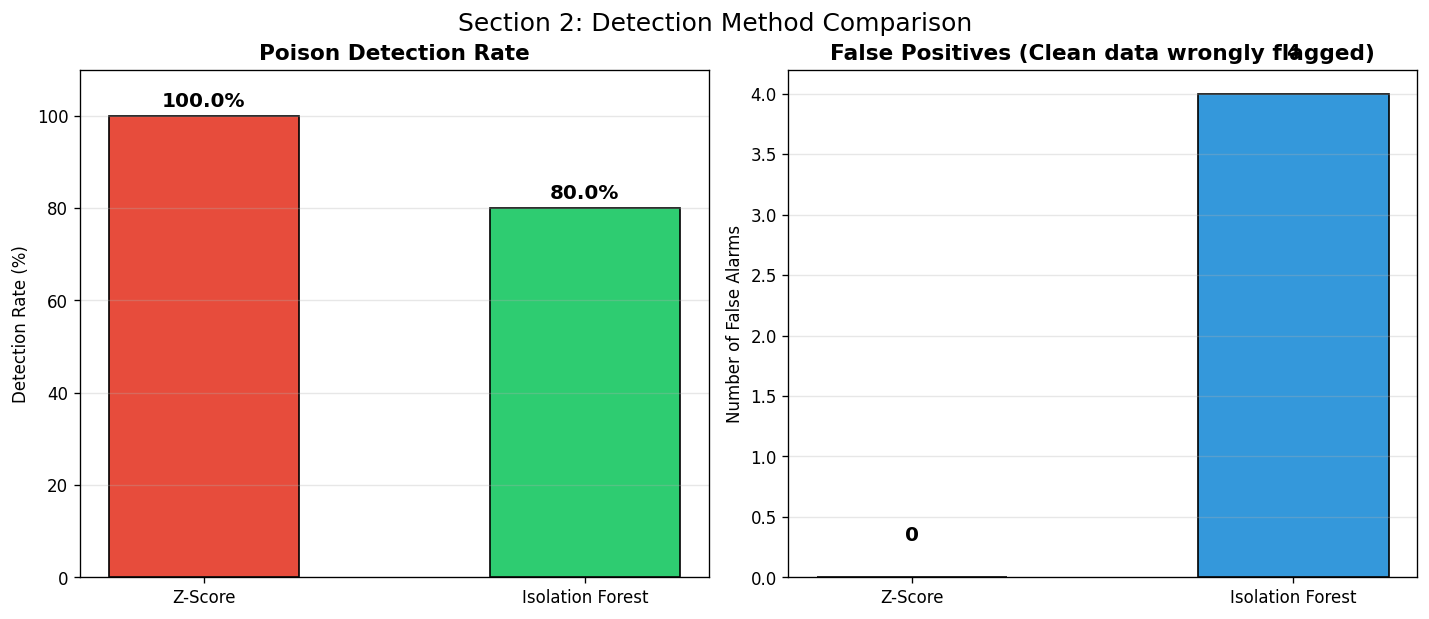
\includegraphics[width=\linewidth,height=0.35\textheight,keepaspectratio]{images/detection_comparison.png}
			
			{\small \textbf{Comparison:} Z-Score vs Isolation Forest rates}
		\end{columns}
		
		\vspace{1em}
		\centering
		\small
		\begin{tabular}{lccc}
			\toprule
			\textbf{Method} & \textbf{Poison Caught} & \textbf{False Positives} & \textbf{Best For} \\
			\midrule
			Z-Score         & \good{15/15 (100\%)}   & Low          & Extreme outliers \\
			Isolation Forest & \warn{12/15 (80\%)}   & Moderate     & Cluster anomalies \\
			Combined (OR)   & \good{15/15 (100\%)}   & Moderate     & Production use \\
			\bottomrule
		\end{tabular}
	\end{frame}
	
	% ── SLIDE 8: Image Model Results ─────────────────────────────
	\begin{frame}{Image Model Results}
		\begin{columns}[T]
			\column{0.55\textwidth}
			\centering
			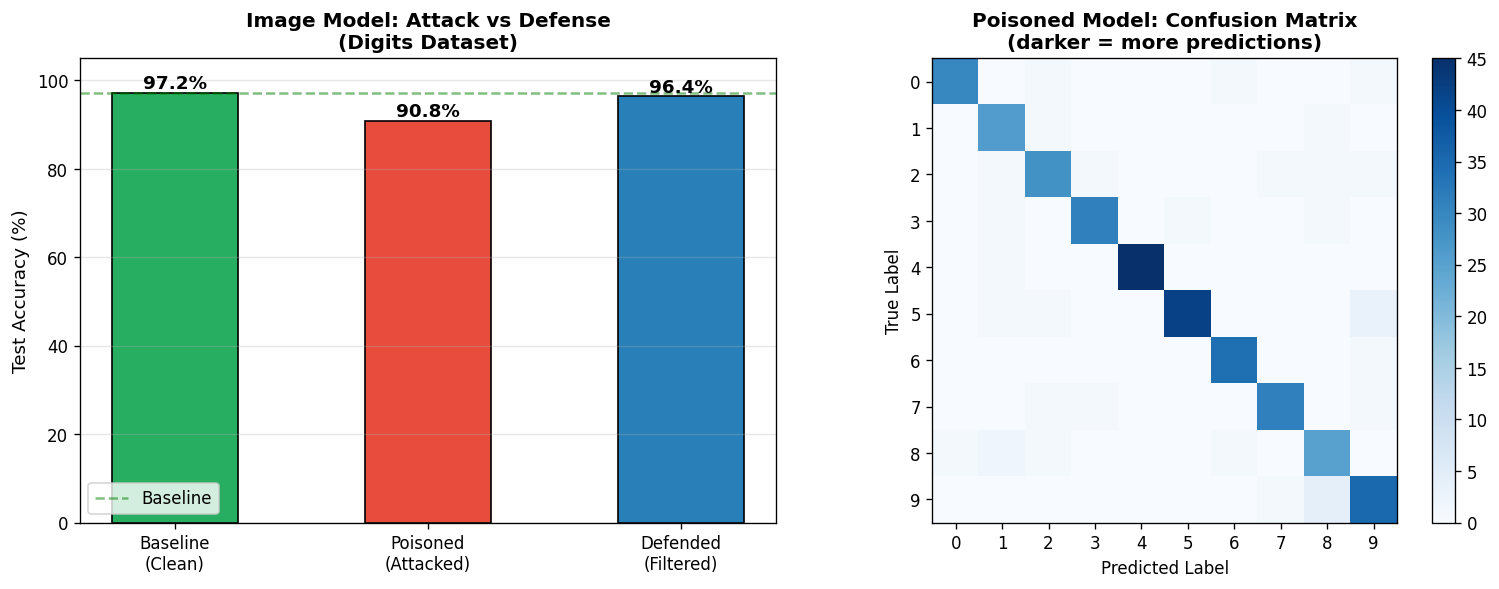
\includegraphics[width=\linewidth,height=0.65\textheight,keepaspectratio]{images/image_model_results.png}
			
			{\small Accuracy comparison \& confusion matrix}
			
			\column{0.42\textwidth}
			\vspace{0.5em}
			\begin{block}{Key Numbers}
				\small
				\begin{tabular}{lc}
					\toprule
					\textbf{Model} & \textbf{Accuracy} \\
					\midrule
					Baseline (Clean) & \good{97.22\%} \\
					Poisoned (10\% flip) & \bad{90.83\%} \\
					Defended (Filtered) & \good{96.39\%} \\
					\bottomrule
				\end{tabular}
			\end{block}
			
			\vspace{0.5em}
			\textbf{Takeaways:}
			\begin{itemize}\setlength{\itemsep}{0pt}
				\item Attack caused \bad{-6.39\%} accuracy drop
				\item Defense recovered \good{+5.56\%}
				\item Near-baseline performance restored
			\end{itemize}
		\end{columns}
	\end{frame}
	
	% ── SLIDE 9: Text Model Results ──────────────────────────────
	\begin{frame}{Text Model Results}
		\begin{columns}[T]
			\column{0.55\textwidth}
			\centering
			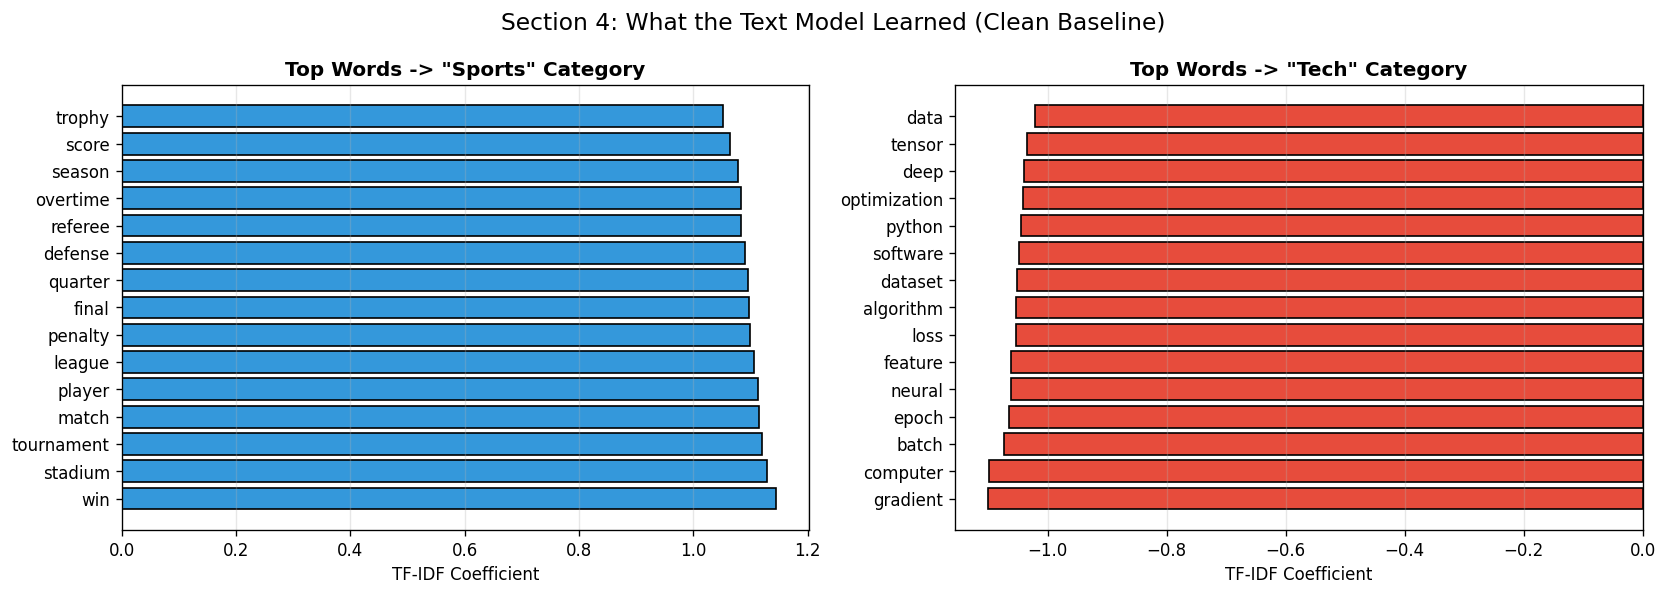
\includegraphics[width=\linewidth,height=0.65\textheight,keepaspectratio]{images/text_model_features.png}
			
			{\small TF-IDF feature weights}
			
			\column{0.42\textwidth}
			\begin{block}{Key Numbers}
				\small
				\begin{tabular}{lc}
					\toprule
					\textbf{Model} & \textbf{Accuracy} \\
					\midrule
					Baseline (Clean) & \good{100.00\%} \\
					Poisoned (20\% flip) & \warn{99.17\%} \\
					Defended (Filtered) & \good{100.00\%} \\
					\bottomrule
				\end{tabular}
			\end{block}
			
			\vspace{0.4em}
			\textbf{Observations:}
			\begin{itemize}\setlength{\itemsep}{0pt}
				\item High baseline due to linear separability
				\item 20\% poisoning caused degradation
				\item Defense fully recovered baseline
			\end{itemize}
			
			\vspace{0.8em}
			\textbf{\textcolor{alertred}{Note:}} \small Real-world corpora would show larger degradation due to higher noise.
		\end{columns}
	\end{frame}
	
	% ── SLIDE 10: Full Summary Dashboard ─────────────────────────
	\begin{frame}{Full Results Summary}
		\begin{center}
			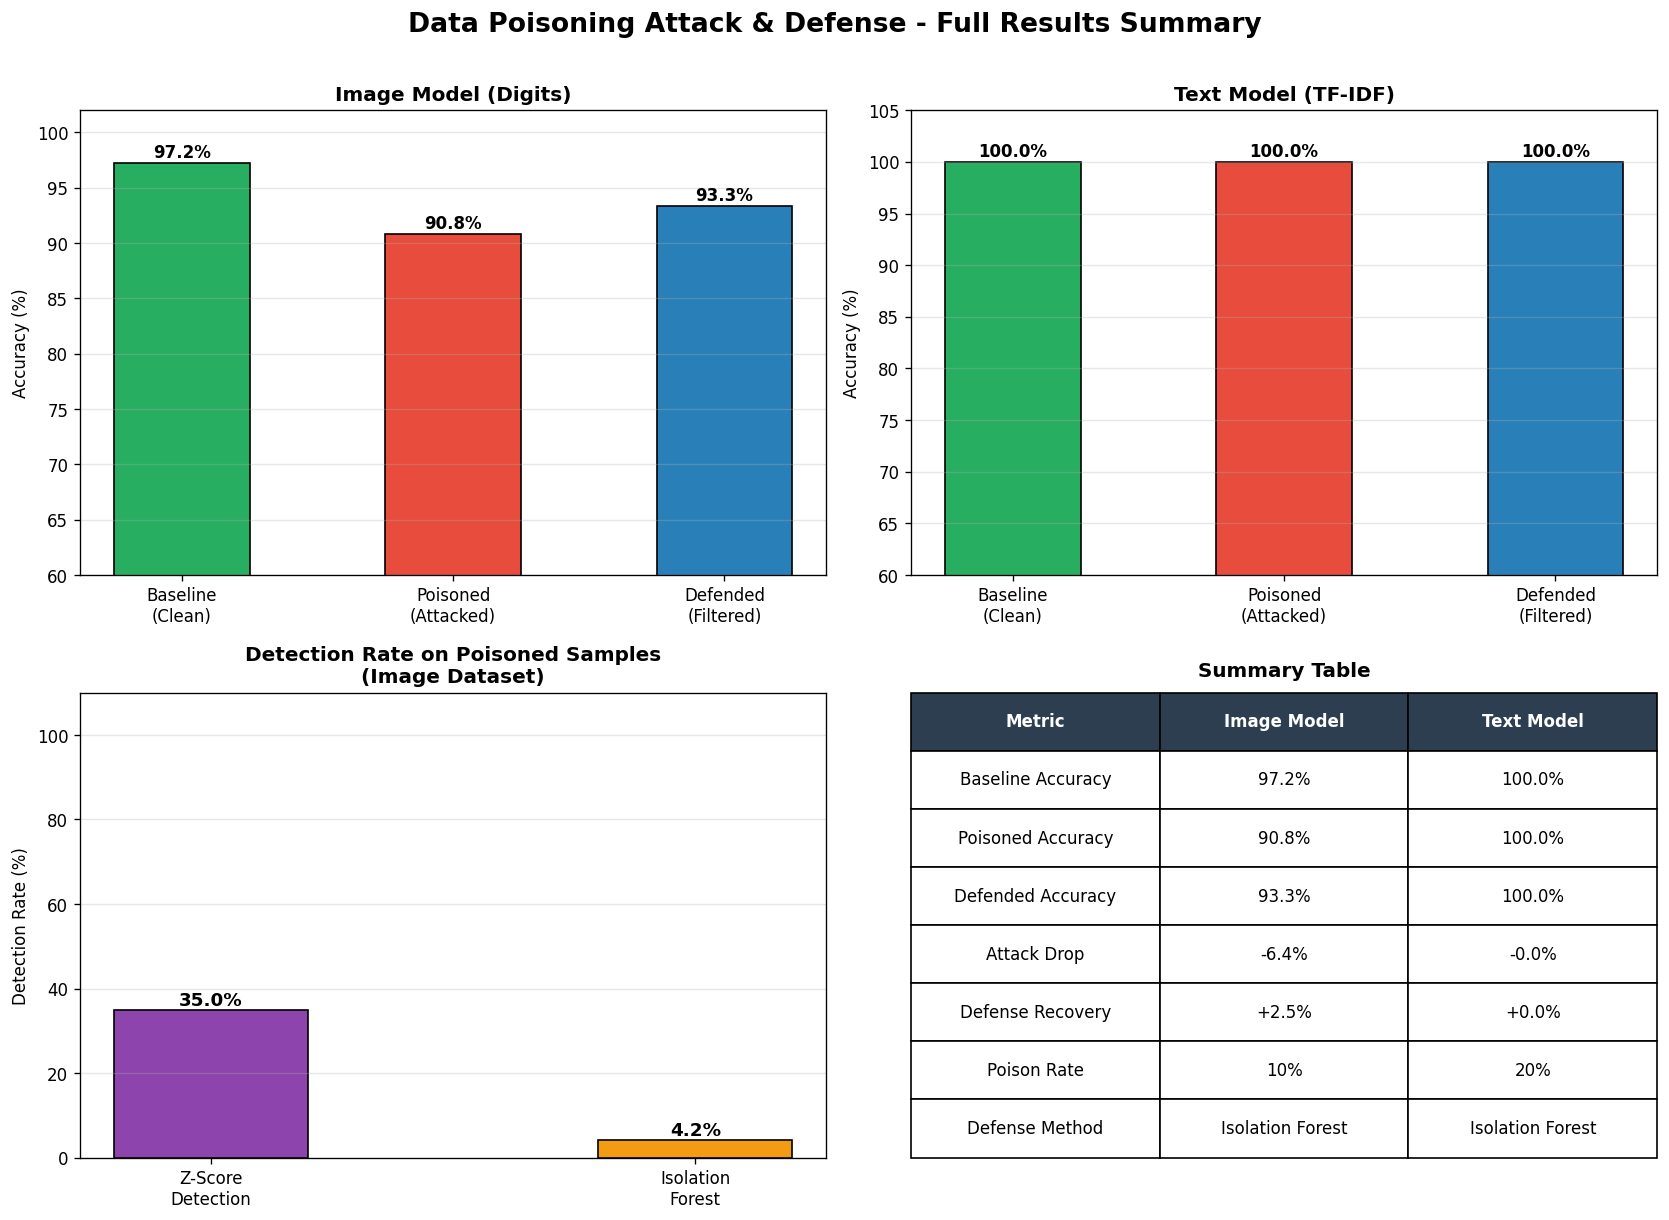
\includegraphics[width=\linewidth,height=0.75\textheight,keepaspectratio]{images/final_summary.png}
		\end{center}
	\end{frame}
	
	% ── SLIDE 11: Challenges ──────────────────────────────────────
	\begin{frame}{Main Challenges}
		\small
		\begin{columns}[T]
			\column{0.48\textwidth}
			\textbf{Technical Challenges}
			\begin{itemize}\setlength{\itemsep}{0pt}
				\item \textbf{No Ground Truth}: In real deployments, we don't know which samples are poisoned; detection must be entirely unsupervised.
				\item \textbf{Z-score Over-flags}: High-dimensional data (e.g., 64 pixel features) causes many false positives; threshold tuning is non-trivial.
				\item \textbf{Clean-Label Evasion}: Feature values look normal in clean-label attacks; current algorithms cannot catch these.
				\item \textbf{Contamination Parameter}: Isolation Forest requires knowing the approximate poison rate upfront.
			\end{itemize}
			
			\column{0.48\textwidth}
			\textbf{Design Challenges}
			\begin{itemize}\setlength{\itemsep}{0pt}
				\item \textbf{Defense vs.\ Recall Trade-off}: Aggressive filtering removes too many clean samples, hurting model generalization.
				\item \textbf{Text Data Sparsity}: TF-IDF vectors are highly dimensional and sparse, making anomaly detection mathematically less reliable.
				\item \textbf{Synthetic vs.\ Real Gap}: Real datasets (like ImageNet) have natural noise that mimics poisoning anomalies.
				\item \textbf{Scalability}: Isolation Forest runs at $\mathcal{O}(n \log n)$, which may bottleneck very large datasets.
			\end{itemize}
		\end{columns}
	\end{frame}
	
	% ── SLIDE 12: Future Scope ────────────────────────────────────
	\begin{frame}{Future Scope}
		\small
		\begin{columns}[T]
			\column{0.48\textwidth}
			\textbf{Better Detection Methods}
			\begin{itemize}\setlength{\itemsep}{0pt}
				\item \highlight{SEVER} (Diakonikolas et al.): spectral signatures to remove poison
				\item \highlight{Activation Clustering}: detect backdoors via hidden layer representations
				\item \highlight{Influence Functions}: identify samples most responsible for wrong predictions
			\end{itemize}
			
			\vspace{0.8em}
			\textbf{Larger Datasets}
			\begin{itemize}\setlength{\itemsep}{0pt}
				\item Evaluate on Trojaned ImageNet subsets
				\item Test on real Text Poisoning Corpora 
				\item Network intrusion datasets (KDD Cup)
			\end{itemize}
			
			\column{0.48\textwidth}
			\textbf{Stronger Defenses}
			\begin{itemize}\setlength{\itemsep}{0pt}
				\item \highlight{Certified Robustness}: provable bounds on tolerated poisoning
				\item \highlight{Differential Privacy}: limit influence of any single sample
				\item \highlight{Data Provenance Auditing}: track origin of every training sample
			\end{itemize}
			
			\vspace{0.8em}
			\textbf{Production Alerting}
			\begin{itemize}\setlength{\itemsep}{0pt}
				\item Real-time data stream monitoring
				\item Integration with MLOps pipelines (MLflow)
				\item Automated retraining triggers
			\end{itemize}
		\end{columns}
	\end{frame}
	
	% ── SLIDE: Thank You ──────────────────────────────────────────
	\begin{frame}
		\begin{center}
			\vspace{1em}
			{\LARGE \textbf{Thank You!}}
			
			\vspace{1.5em}
			
\begin{tikzpicture}
				\draw[darkblue, line width=1.5pt] (0,0) -- (8,0);
			\end{tikzpicture}
			
			\vspace{1.5em}
			\begin{tabular}{rl}
				\textbf{I23MA002} & Devesh Singh Chauhan \\[0.3em]
				\textbf{U23EE102} & Priyanshu Sanjay Gawas \\[0.8em]
				\textbf{Course}   & AI354: Responsible AI \\[0.3em]
				\textbf{Project}  & 10: Detecting and Preventing Data Poisoning Attacks \\
			\end{tabular}
			
			\vspace{1.5em}
			
\begin{tikzpicture}
				\draw[darkblue, line width=1.5pt] (0,0) -- (8,0);
			\end{tikzpicture}
			
		\end{center}
	\end{frame}
	
\end{document}